\section{A New Approach}
While the Gaussian splatting method is very impressive, this section will discuss a potential new path for \gls{nvs} inspired by the Gaussian splatting method.
The core idea is to leverage the power of hardware-accelerated ray tracing and replace the current rasterization pipeline with a ray tracing pipeline.
Additionally, the use of polarization cameras might prove useful in this regard, as reflected light has a distinct polarization signature \cite{lingUniversityPhysicsVolume2016}.
This


\subsection{Ray Tracing}
Ray tracing is a rendering technique that simulates how rays of light traverse a scene.
Unlike rasterization, which confines rendering to a single viewpoint at a time by projecting the scene onto a two-dimensional image plane, ray tracing can simultaneously render rays originating from multiple viewpoints \cite{caulfieldWhatPathTracing2022}.
This capability empowers ray tracing programs to simulate lifelike lighting scenarios by estimating how light scatters and reflects off objects in the scene \cite{caulfieldWhatPathTracing2022}.

As ray tracing has become a key component of rendering in the video game industry, specialized hardware has been developed to accelerate the process to achieve real-time performance.
Modern NVIDIA GPUs have dedicated \gls{rt} cores that can be used to accelerate ray tracing through the NVIDIA OptiX\textsuperscript{TM} API \cite{nvidiaNVIDIAOptiXProgramming2023}.

The main computational bottleneck of ray tracing is finding the intersections between the rays and the scene geometry.
To speed up this process, a \gls{bvh} is used to store the scene geometry \cite{nvidiaNVIDIAOptiXProgramming2023}.
A \gls{bvh} is a tree data structure that recursively divides the scene into smaller and smaller bounding boxes making it possible to quickly discard large parts of the scene that the ray does not intersect with \cite{nvidiaNVIDIAOptiXProgramming2023}.
The \gls{rt} cores are specialized hardware that can traverse the \gls{bvh} and find the first intersection between a ray and the objects in the scene \cite{nvidiaNVIDIAOptiXProgramming2023}.

\subsection{Triangle Representation}
While Optix supports custom primitive types, making the use of Gaussians possible, operations on custom primitives are not only partially accelerated by the \gls{rt} cores \cite{nvidiaOptiXQuickStart2018}\cite{nvidiaNVIDIAOptiXProgramming2023}.
This makes the use of triangles a more attractive option.
The implementation in the paper projects the Gaussians onto the image plane, so they are not performing any volumetric rendering.
This makes it likely that using triangles should also be possible.



Another small advantage of using triangles is the ability to perform backface culling, where triangles facing away from the camera are discarded, reducing the number of triangles that have to be tested for intersection.

\begin{figure}
    \centering
    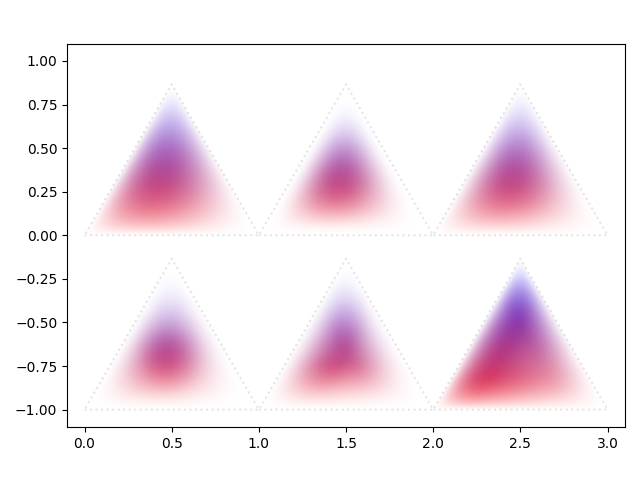
\includegraphics[width=\linewidth]{images/alphas.png}
    \caption{Experimentation with different polynomial functions on barycentric coordinate values to obtain a smooth opacity function. The lower right vertex of each triangle has opacity 0 to test vertex-dependent opacity.}
    \label{fig:alphas}
\end{figure}

\subsection{Remove Popping Artifacts}
As discussed, a key issue with the current implementation is popping artifacts where Gaussians suddenly appear or disappear behind other Gaussians.
Raytracing will solve most of this issue as the projection approximation described in Section \ref{sec:projection} is no longer needed.
Still, in the intersection area between two triangles, the gradients will be discontinuous due to how alpha blending works, as shown in Equation \ref{eq:alpha_blending}.

A potential approach to solving this and achieving a smooth transition when triangles move through each other,
is to use a dynamic alpha blending function where the ray distance between the current triangle intersection and the previous triangle intersection is taken into account.
This does however appear to create a lot of dependence between the triangles, as the alpha value of each triangle is dependent on the alpha value of the next triangle which is dependent on the alpha value of the next triangle and so on.


\subsection{Inter Triangle Regularization}
A key benefit of capturing the intersections between rays and triangles is that we can perform inter-triangle regularization.
For each intersection point with a triangle, we can capture information about the distance and color of the previous and next intersection points.
If the distances are within some adaptive threshold, we can add a regularization term to the loss function, such that neighboring triangles should stick together.
Hopefully, this will help towards having smoother surfaces and aligning the face normal of neighboring triangles.

\subsection{Reflections}
Reflections in the scene pose a significant challenge in the field of \gls{nvs}, as it requires the ability to capture view-dependent color.
As discussed earlier, the use of spherical harmonics solves this to some degree, but it comes at a significant memory cost.
When using ray tracing, it might be possible to circumvent the need for view-dependent color by using ray-traced reflections.

Without the use of ray tracing cores, this is impossible, as the whole rendering pipeline for the Gaussian splats, discussed in Section \ref{sec:rasterization}, would have to be performed for each reflected ray as they would not share the same origin.
This would make the rendering process several million times slower.
But with the use of ray tracing cores, rendering a reflected ray is no different than rendering a regular ray \footnote{It might be slightly worse due to data locality, but this should be handled by the hardware.}.

It is however still very likely that it is infeasible to optimize the scene with reflections.
A core reason for this is that it is very expensive to capture glossy reflections, such as light reflected from a table surface, as statistical sampling with a large number of sample rays is required to get a good result.
Another key challenge is that a very small change in the orientation of a triangle can have large effects on the reflected light, resulting in very sharp gradients.


\subsection{Leverage Polarization}

, as reflected light has a distinct polarization signature \cite{lingUniversityPhysicsVolume2016}.


The simple approach would be to remove reflected light from the scene and partially circumvent the need for view-dependent color.
This approach only targets the input data and should thus be easy to evaluate using the implementation from the paper.
The results from this approach will however look different than what a regular camera would capture, as the reflected light is partially removed.

Another, arguably more interesting, approach would be to use the polarization information to estimate the surface normal of each triangle and calculate ray-traced reflections.
As the polarization cameras can capture the angle of polarization for each pixel, using multiple views it should be possible to estimate the three-dimensional surface normals with some degree of accuracy.
This approach has been presented by one manufacturer of polarization cameras as shown in Figure \ref{fig:polarization} \cite{lucidvisionlabs3DDepthSurface2021}.


\begin{figure}
    \centering
    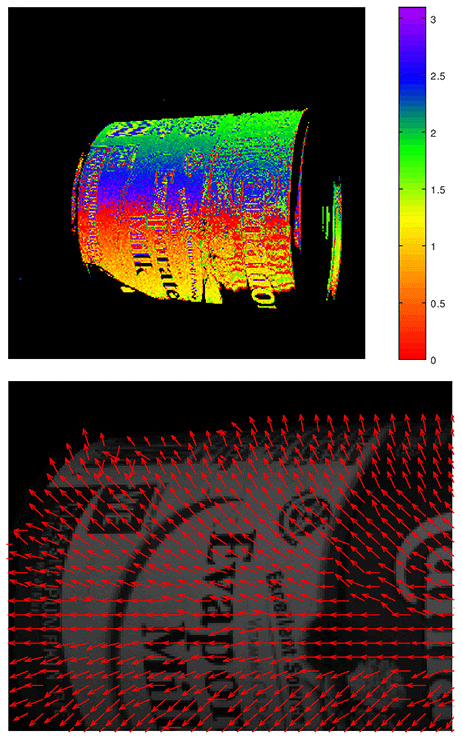
\includegraphics[width=\linewidth]{images/polarization_normals.png}
    \caption{Angle of orientation and estimated surface normals from polarized light \cite{lucidvisionlabs3DDepthSurface2021}}.
    \label{fig:polarization}
\end{figure}






\subsection{Code closer to Problem formulation}
There is a significant difference between how the problem is formulated in the paper and how